\documentclass[main]{subfiles}

\begin{document}

\tableofcontents
\newpage

\section{Homotopy}

\begin{definition}
$\pi_n(X):=[S^n,X]$ are the homotopy groups, the relative homotopy groups $\pi_n(X,A)$ are defined to be all homotopy classes of maps $(I^n,\partial I^n)\to(X,A)$ or equivalently all homotopy classes of maps $(S^n,s_0)\to(X,A)$, in particular, if $A=\{x_0\}$, we have $\pi_n(X,x_0):=\langle S^n,X\rangle$ with basepoints $x_0,s_0$, furthermore, we also define $\pi_n(X,A,x_0)$ to be all homotopy classes of maps $(I^n,\partial I^n,J^{n-1})\to(X,A,x_0)$ or equivalently all homotopy classes of maps $(D^n,S^{n-1},s_0)\to(X,A,x_0)$, here $J^{n-1}=\partial I^n-I^{n-1}$ \par
$\pi_1(X,x_0)$ is called the fundamental group, note that $\pi_n(X,x,x)=\pi_n(X,x)$
\end{definition}

\begin{definition}
All homotopy classes of paths form the \textit{fundamental groupoid}\index{Fundamental groupoid} $\Pi_1(X)$ of $X$, suppose $A\subseteq X$, we can also define $\Pi_1(X,A)$ to be the full subcategory with objects $x\in A$ and morphisms $\Hom(x,y),x,y\in A$, $\Pi_1(X,x)=\pi_1(X,x)$, $\Pi_1(X)$ is a connected category if $X$ is path-connected since there is a morphism connecting any two objects, thus $\pi_1(X,x)$ is a skeleton of $\Pi_1(X)$, $\pi_1(X,x)\hookrightarrow\Pi_1(X)$ is an equivalence of categories
\end{definition}

\begin{proposition}
$\pi_n(X,x_0)$ are groups, abelian if $n>1$
\end{proposition}

\begin{theorem}[Van Kampen's theorem]\label{Van Kampen's theorem}
Suppose $X=\displaystyle\bigcup_{\alpha}A_\alpha$, interiors of $A_\alpha$ cover $X$, where $X,A_\alpha,A_\alpha\cap A_\beta$ are path connected and $x_0\in A_\alpha$, then the map induced by inclusion $\underset{\alpha}{*}\pi_1(A_\alpha,x_0)\to\pi_1(X,x_0)$ is surjective. Moreover, if $A_\alpha\cap A_\beta\cap A_\gamma$ are path connected, then then kernel is generated by $i_\alpha(w)i_\beta(w)^{-1},w\in\pi_1(A_\alpha\cap A_\beta,x_0)$, where $i_\alpha:A_\alpha\to X$ are the inclusions
\end{theorem}

\begin{proof}
Since $A_\alpha\cap A_\beta$ are path connected, we can cut a loop in $X$ into pieces such that each intermediate point is in $A_\alpha\cap A_\beta$ for some $\alpha,\beta$, thus the map is surjective \par
Suppose $f_1\cdots f_n$, $g_1\cdots g_m$ are homotopic as loops, suppose $F$ is the homotopy, consider the following diagram, each rectangle is so small that it is inside some $A_\alpha$, then homotopy the path across a cube one at a time, and since $A_\alpha\cap A_\beta\cap A_\gamma$ are path connected, each vertex lies in $A_\alpha\cap A_\beta\cap A_\gamma$ for some $\alpha,\beta,\gamma$, then we can connected it to $x_0$ through a path in $A_\alpha\cap A_\beta\cap A_\gamma$
\begin{center}
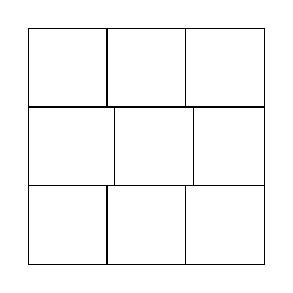
\begin{tikzpicture}
\draw (0,0)--(3,0)--(3,3)--(0,3)--cycle;
\draw (0,1)--(3,1);
\draw (0,2)--(3,2);
\draw (1,1)--(1,0);
\draw (2,1)--(2,0);
\draw (1,3)--(1,2);
\draw (2,3)--(2,2);
\draw (1.1,2)--(1.1,1);
\draw (2.1,2)--(2.1,1);
\end{tikzpicture}
\end{center}
\end{proof}

\begin{theorem}
$X$ is a path-connected, attach cells $\{e^2_\alpha\}$ along loops
\end{theorem}

\begin{definition}
$X\xrightarrow f Y$ is a \textbf{weak homotopy equivalence}\index{Weak homotopy equivalence} if $\pi_0(X,x_0)\xrightarrow{f_*}\pi_0(Y,f(x_0))$ is bijective, and on each path connected component, $\pi_n(X,x_0)\xrightarrow{f_*}\pi_n(Y,f(x_0))$ are isomorphisms
\end{definition}

\begin{theorem}[Hurewicz theorem]\label{Hurewicz theorem}
Choose a generator $e\in H_n(S^n)$, define $\phi:\pi_n(X)\to H_n(X)$, $f\mapsto f_*(e)$, here $f:S^n\to X$ is a map. If $X$ is $ (n-1)$-connected, then $\phi$ is an isomorphism
\end{theorem}



\section{Hurewicz fibration}

\begin{definition}
$E\xrightarrow{p}B$ is a \textbf{Hurewicz fibration}\index{Hurewicz fibration} if it has homotopy lifting property for any space $X$
\begin{center}
\begin{tikzcd}
X \arrow[r] \arrow[d,hook] & E \arrow[d,"p"] \\
X\times I \arrow[ur,dashed] \arrow[r] &B
\end{tikzcd}
\end{center}
$p^{-1}(A)\xrightarrow{p} A$ is also a fibration for any $A\subseteq B$
\end{definition}

\begin{definition}
$A\xrightarrow{i}X$ is a \textbf{Hurewicz cofibration}\index{Hurewicz cobfibration} if for any $X\xrightarrow{f_0}Y$, $A\times I\xrightarrow{g}Y$ such that $g_0=f_0i$, there there exists $X\times I\xrightarrow{f}Y$ extends $f_0$ such that $g=fi$
\begin{center}
\begin{tikzcd}
Y             & X \arrow[l, "f_0"'] \arrow[ld, "f"', dashed] \\
Y^I \arrow[u] & A \arrow[u, "i"'] \arrow[l, "g"]          
\end{tikzcd}
\end{center}
By Lemma \ref{Cofibration is an embedding}, $A\hookrightarrow X$ is an embedding, $(X,A)$ is a \textbf{cofibered pair}\index{Cofibered pair} satisfying the \textbf{homotopy extension property}\index{Homotopy extension property}
\end{definition}

\begin{remark}
The fiber of a fibration is the kernel in $Top$. The cofiber $X/A$ of a cofibration is the cokernel in $Top$ \par
$A\times I$ can be thought of as the "continuous" coproduct $\displaystyle\coprod_iA$, and $A^I$ can be thought of as the "continuous" product $\displaystyle\prod_iA$
\end{remark}

\begin{lemma}\label{Cofibration is an embedding}
Cofibration $A\xrightarrow{i}X$ is a topological embedding
\end{lemma}

\begin{proof}
$M$ is the mapping cylinder of $A\xrightarrow{i}X$, $X\times\{0\}\sqcup A\times I\xrightarrow{[\,]}M$ denote the quotient map, $f_0(x)=[(x,0)]$, $g_t(a)=[(a,t)]$, then $g_0(a)=[(a,0)]=[(i(a),0)]=f_0i(a)$
\begin{center}
\begin{tikzcd}
M             & X \arrow[l, "f_0"'] \arrow[ld, "f"', dashed] \\
M^I \arrow[u] & A \arrow[u, "i"'] \arrow[l, "g"]            
\end{tikzcd}
\end{center}
$M|_{A\times\{1\}}\xrightarrow{k}A$, $[(a,1)]\mapsto a$ is a homeomorphism, $kf_1|_{i(A)}$ is the inverse of $i$ because $kf_1i(a)=kg_1(a)=k([(a,1)])=a$, $ikf_1(i(a))=i(a)$
\end{proof}

\begin{lemma}
A surjective fibration $E\xrightarrow{p}B$ with $B$ locally path connected is a quotient map
\end{lemma}

\begin{lemma}\label{Mapping cylinder of inclusion has subspace topology if it is a retraction}
If $X\times\{0\}\cup A\times I$ is a retract of $X\times I$, then the topology of the mapping cylinder of the inclusion $A\hookrightarrow X$ is the the same as the subspace topology on $X\times\{0\}\cup A\times I$ induced from $X\times I$. In particular, $f$ is continuous on $X\times\{0\}\cup A\times I$ iff $f$ is continuous on both $X\times\{0\}$ and $A\times I$
\end{lemma}

\begin{proof}
This is trivial if $A$ is closed due to Lemma \ref{Pasting lemma} \par
Write $Y=X\times\{0\}\cup A\times I$. If $O\subseteq Y$ is open in $Y$, then obviously $O\cap A\times I$ is open in $A\times I$, $O\cap X$ is open in $X$ \par
Suppose $O\subseteq Y$ is such that $O\cap A\times I$ is open in $A\times I$, $O\cap X$ is open in $X$. Define  $\displaystyle U_n=\bigcup_V\left\{V\overset{\mathrm{open}}{\subseteq}X\middle|(V\cap A)\times[0,\textstyle\frac{1}{n})\subseteq O\right\}$, i.e. $U_n$ is the largest such open subset of $X$, $U=\bigcup_{n=1}^\infty U_n$, then $O\cap A\subseteq U$ since for any $(x,0)\in O\cap A\subseteq O\cap A\times I$, because $O\cap A\times I$ is open $A\times I$, there exists open subset $V\subseteq X$ containing $x$ such that $(V\cap A)\times[0,\frac{1}{n})\subseteq O\cap A\times I$ for some $n$, hence $x\in V\subseteq U_n\subseteq U$ \par
$O\cap A\times(0,1]$ is open in $Y$, $O\cap(X\setminus\overline A)$ is open in $Y$, we only need to show that for any $x\in\overline A$, there exists an open neighborhood of $(x,0)$ contained in $O$, and it suffices to show that $x\in U$, then $x\in U_n$ for some $n$, $(U_n\cap O)\times[0,\frac{1}{n})\cap Y$ is open in $Y$. Now fix $x\in\overline A$ \par
Write the retraction $r$ as $(r_1,r_2)$, for $t>0$, $r(x,t)=(r_1(x,t),r_2(x,t))$, since $x\in\overline A$, $r(a,t)=(a,t)$, we know $r_1(x,t)\in A$, $r_2(x,t)=t$. We claim: if $r_1(x,t)\in U_n$, then $x\in U_n$. Since $U_n$ is open, there exists open neighborhood $V$ of $x$ such that $r_1(V\times(t-\varepsilon,t+\varepsilon))\subseteq U_n$ for some $\varepsilon>0$, in particular $r_1((V\cap A)\times\{t\})\subseteq U_n$, thus $V\cap A\subseteq U_n\cap A$, by maximality of $U_n$, $V\subseteq U_n$ \par
Suppose $x\notin U$, then by the claim, $r_1(x,t)\in A\setminus U$ for $t>0$, then $r_1(x,t)\in A\setminus O$ since $A\cap O\subseteq U$, thus $x=r_1(x,0)\in\overline A\setminus O$ which contradicts the fact $(x,0)\in A$
\end{proof}

\begin{proposition}\label{A->X is a cofibration iff retraction exists}
$(X,A)$ is cofibered iff $X\times\{0\}\cup A\times I$ is a retract of $X\times I$ iff $X\times\{0\}\cup A\times I$ is a strong deformation retract of $X\times I$
\end{proposition}

\begin{proof}
If $A\xrightarrow{i}X$ is a cofibration, then $X\times\{0\}\cup A\times I\xrightarrow{1}X\times\{0\}\cup A\times I$ induces a retraction. Conversely, by Lemma \ref{Mapping cylinder of inclusion has subspace topology if it is a retraction}, $A\times I\xrightarrow{g}Y$, $X\xrightarrow{f_0}Y$ with $g_0=f_0|_A$ gives a map $X\times\{0\}\cup A\times I\to Y$, composing with retraction gives $X\times I\to Y$ \par
A strong deformation retraction is given by $H((x,t),s)=(\Pr_X r(x,st),s\Pr_Ir(x,t)+(1-s)t)$
\end{proof}

\begin{lemma}
If $(X,A)$ is cofibered, so is $(X,\overline A)$
\end{lemma}

\begin{proof}
Define $\displaystyle\phi(x)=\inf_{t\in I}\{\textstyle\Pr_Ir(x,t)\neq0\}$, then there is a retraction $X\times I\xrightarrow{r'}X\times\{0\}\cup\overline A\times I$
\[r'(x,t)=\begin{cases}
\left(\Pr_Xr(x,t),0\right) &t\leq\phi(x) \\
\left(\Pr_Xr(x,\phi(x)),t-\phi(x)\right) &t\geq\phi(x)
\end{cases}\]
\end{proof}

\begin{lemma}\label{p:E->B fibration, i:A->X strong deformation retract, A can be perfectly separated => i has LLP}
$E\xrightarrow{p}B$ is a fibration, $A$ is a strong deformation retract of $X$ and $A$ can be perfectly separated, then
\begin{center}
\begin{tikzcd}
A \arrow[r, "f''"] \arrow[d, "i"', hook]   & E \arrow[d, "p"] \\
X \arrow[ru, "f", dashed] \arrow[r, "f'"'] & B               
\end{tikzcd}
\end{center}
$f$ is unique up to homotopy $\mathrm{rel}A$
\end{lemma}

\begin{proof}
$X\xrightarrow{\phi}\mathbb R$ is a function such that $\phi^{-1}(0)=A$. $X\xrightarrow{r}A$ is the retract. $X\times I\xrightarrow{D} X$ is a homotopy from $ir$ to $1_X$. Define $H(x,t)=\begin{cases}
D(x,t/\phi(x)) &t\leq\phi(x) \\
D(x,1) &t\geq\phi(x)
\end{cases}$
\begin{center}
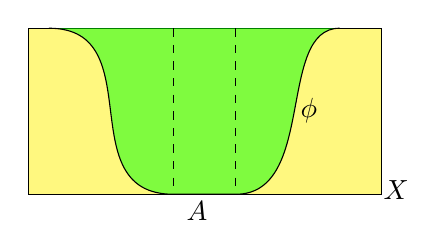
\begin{tikzpicture}[x=0.75pt,y=0.75pt,yscale=-1,xscale=1]
\draw  [fill=yellow  ,fill opacity=0.5 ] (100,90) -- (270,90) -- (270,170) -- (100,170) -- cycle ;
\draw [fill=green  ,fill opacity=0.5 ]   (110,90) .. controls (159.57,90) and (119.57,170) .. (170,170) .. controls (220.43,170) and (161,170) .. (200,170) .. controls (239,170) and (219.57,90) .. (250,90) ;
\draw [dashed]   (170,90) -- (170,170) ;
\draw  [dashed]  (200,90) -- (200,170) ;
\draw (230,122.4) node [anchor=north west][inner sep=0.75pt]    {$\phi $};
\draw (270,162) node [anchor=north west][inner sep=0.75pt]    {$X$};
\draw (175,172.4) node [anchor=north west][inner sep=0.75pt]    {$A$};
\end{tikzpicture}
\end{center}
Since $E\xrightarrow pB$ is a fibration, we have a lift $X\times I\xrightarrow FE$ such that $pF=f'H$ and $F_0=f''r$ because $pF_0=pf''r=f'ir=f'H_0$. Define $f$ to be the composition $X\xrightarrow{1\times\phi}X\times I\xrightarrow{F}E$, then we have $fi=F(1\times\phi)=F_0i=f''$ and $pf=pF(1\times\phi)=f'H(1\times\phi)=f'D_1=f'$
\begin{center}
\begin{tikzcd}
X \arrow[r, "r", shift left] \arrow[d, hook]       & A \arrow[r, "f''"] \arrow[l, "i", hook, shift left]       & E \arrow[d, "p"] \\
X\times I \arrow[rru, "F", dashed] \arrow[r, "H"'] & X \arrow[r, "f'"'] \arrow[l, "1\times\phi", bend left=49] & B               
\end{tikzcd}
\end{center}
\end{proof}

\begin{proposition}\label{Fibrations have homotopy lifting property for closed cofibrations}
Fibrations have homotopy lifting property for closed cofibrations
\begin{center}
\begin{tikzcd}
X\times\{0\}\cup A\times I \arrow[r] \arrow[d, "i"', hook] & E \arrow[d, "p"] \\
X\times I \arrow[ru, dashed] \arrow[r]     & B               
\end{tikzcd}
\end{center}
\end{proposition}

\begin{proposition}
If $(X,A)$, $(Y,B)$ are cofibered, $A\subseteq X$ is closed, then $(X\times Y,X\times B\cup A\times Y)$ is also cofibered. If in addition $A$ or $B$ is a strong deformation retract of $X$ or $Y$, then $X\times B\cup A\times Y$ is a strong deformation retract of $X\times Y$
\end{proposition}

\begin{proposition}\label{Fibers of fibration are homotopy equivalent}
$E\xrightarrow{p}B$ is a fibration, then the fibers over connected components of $B$ are homotopic. More over, for any path $\gamma:I\to B$, we can get a lifting $g_t:F_{\gamma(0)}\to F_{\gamma(t)}$ of $F_{\gamma(0)}\hookrightarrow E$, define $L_\gamma:F_{\gamma(0)}\to F_{\gamma(1)}$ to be $g_1$, if $\gamma\simeq\eta$ rel $\partial I : I\to B$, then $L_\gamma\simeq L_\eta$, and for any $\gamma,\eta:I\to B$, $\eta(0)=\gamma(1)$, $L_{\gamma\eta}\simeq L_\gamma L_\eta$
\end{proposition}

\begin{proof}
According to homotopy lifting property, lifting up $A\times F_{\gamma(0)}\to E$ is homeomorphic to $B\times F_{\gamma(0)}\to E$
\end{proof}

\begin{remark}
We can think of this as an action of $\pi_1(B)$ on $H_*(F)$
\end{remark}

\begin{definition}
$E_1\xrightarrow{p_1}B_1$, $E_2\xrightarrow{p_2}B_2$ are fibrations, $p_1\xrightarrow{f_0,f_1} p_2$ are \textbf{fiber homotopic}\index{Fiber homotopy} if there exists $p_1\xrightarrow{f_t} P_2$ varying from $f_0$ to $f_1$. $p_1,p_2$ are \textbf{fiber homotopy equivalent}\index{Fiber homotopy equivalence} if there are fiber homotopies $p_0\xrightarrow{f}p_1$ and $p_1\xrightarrow{g}p_0$ such that $fg$, $gf$ fiber homotopic to $1$
\end{definition}

\begin{lemma}\label{i:A->B cofibration is homotopy equivalence iff A strong deformation retract}
Cofibration $A\xrightarrow{i}X$ is a homotopy equivalence iff $A$ is a strong deformation retract of $X$. Fibration $E\xrightarrow{p}B$ is a homotopy equivalence iff there exists a section $B\xrightarrow{s}E$ such that $sp$ is fiber homotopic to $1$
\end{lemma}

\begin{proof}
If $i$ is a homotopy equivalence, then there exists $X\xrightarrow {r'}A$ such that $ir'\simeq1_X$, $r'i\simeq1_A$, by Lemma \ref{Some rudimentary lemma about retract and deformation}, since $(X,A)$ is cofibered, $r'\simeq r$ is a retract and then $A$ is a deformation retract of $X$. Suppose $X\times I\xrightarrow FX$ is a homotopy from $1_X$ to $ir$ \par
$\Gamma=X\times\{0\}\cup A\times I\cup X\times\{1\}=X\times\{0\}\cup A\times[0,\frac{1}{2}]\cup A\times [\frac{1}{2},1]\cup X\times\{1\}$ is a retract of $X\times I$. Construct $\Gamma\times I\xrightarrow GX$
\[G((x,t),s)=\begin{cases}
F(x,(1-s)t) &(x,t)\in X\times\{0\}\cup A\times I \\
F(r(x),1-s) &(x,t)\in X\times\{1\}
\end{cases}\]
$G_1$ can be extends to $X\times I\xrightarrow HX$, then $H_0(x)=G_1(x,0)=F(x,0)=x$, $H_1(x)=G_1(x,1)=F(r(x),0)=r(x)$, $H_t(a)=G_1(a,t)=F(a,0)=a$, i.e. $H$ is a strong deformation retraction
\end{proof}

\begin{lemma}\label{fibration map is a homotopy equivalence iff it is a fiber homotopy equivalence}
$E\xrightarrow{p}B$ is a fibration, $A\xrightarrow{f} B$ is a map, $A\times_B E=f^*(E)$ is the \textbf{pullback fibration}, suppose $f_t:A\to B$ is a homotopy, then pullback fibrations $f_0^*(E)\to A$, $f_1^*(E)\to A$ are fiber homotopy equivalent. In particular, a morphism $p\xrightarrow{f}q$ between two fibrations is a homotopy equivalence iff $f$ is a fiber homotopy equivalence
\end{lemma}

\begin{proof}
$A\times I\xrightarrow{F} B$ is a homotopy, we have the pullback fibration $F^*(E)$, it suffices to show that for any fibration $E\xrightarrow{p}B\times I$, $E_0:=p^{-1}(B\times\{0\})\simeq p^{-1}(B\times\{1\})=:E_1$ are fiber homotopy equivalent \par
Consider the following diagrams
\begin{center}
\begin{tikzcd}
E_0\arrow[r,hook]\arrow[d,hook] &E \arrow[d,"p"] \\
E_0\times I \arrow[r,"{(p,t)}"'] \arrow[ur,dashed] &B\times I
\end{tikzcd}
\end{center}
\begin{center}
\begin{tikzcd}
E_1\arrow[r,hook]\arrow[d,hook] &E \arrow[d,"p"] \\
E_1\times I \arrow[r,"{(p,1-t)}"'] \arrow[ur,dashed] &B\times I
\end{tikzcd}
\end{center}
Then we get fiber preserving maps $f:E_0\to E_1$ and $g:E_1\to E_{0}$, and restricts them to each fiber
\begin{center}
\begin{tikzcd}
p^{-1}(b,0)\arrow[r,hook]\arrow[d,hook] &E \arrow[d,"p"] \\
p^{-1}(b,0)\times I \arrow[r,"{(p,t)}"'] \arrow[ur,dashed] &\{b\}\times I
\end{tikzcd}
\end{center}
\begin{center}
\begin{tikzcd}
p^{-1}(b,1)\arrow[r,hook]\arrow[d,hook] &E \arrow[d,"p"] \\
p^{-1}(b,1)\times I \arrow[r,"{(p,1-t)}"'] \arrow[ur,dashed] &\{b\}\times I
\end{tikzcd}
\end{center}
We get maps $f|_{p^{-1}(b,0)}:p^{-1}(b,0)\to p^{-1}(b,1)$, $g|_{p^{-1}(b,1)}:p^{-1}(b,1)\to p^{-1}(b,0)$, according to Proposition \ref{Fibers of fibration are homotopy equivalent} they are homotopy equivalence and inverses to each other, hence $f,g$ are fiber homotopy equivalences and inverses to each other
\end{proof}

\begin{corollary}
$E\xrightarrow{p}B$ is a fibration, $B$ contractible, then $p$ is fiber homotopy equivalent to $B\times F\to B$. If $B$ is locally contractible, the fibration is locally homotopy equivalent to a product
\end{corollary}

\begin{proof}
Since $B$ is contractible, identity map is homotopic to a constant map, and the pullback of $E$ under the identity map is $E$ itself, the pullback of $E$ under a constant map is fiber bundle $B\times F$
\end{proof}

\begin{definition}
$(X,x_0)$ is a pointed space. The \textbf{loop space}\index{Loop space} $\Omega X$ consists of all the loops on $X$ starting and ending at $x_0$, the constant loop being the basepoint. The \textbf{path space}\index{path space} $PX$ consists of all the paths starting at $x_0$. $\Omega X\subseteq PX\subseteq X^I$ endowed with the subspace topology
\end{definition}

\begin{proposition}
$\langle\Sigma X,Y\rangle=\langle X,\Omega Y\rangle$ is an adjunction
\end{proposition}

\begin{definition}
The \textbf{mapping path space} $P_f$ is the pullback
\begin{center}
\begin{tikzcd}
P_f \arrow[d] \arrow[r] & Y^I \arrow[d] \\
X \arrow[r, "f"]        & Y                      
\end{tikzcd}
\end{center}
$P_f$ deformation retracts onto $X$ by shrinking paths.
The \textbf{homotopy fiber} $F_f$ of $f$ over $y$ is the pullback
\begin{center}
\begin{tikzcd}
F_f \arrow[d] \arrow[r] & Y^I \arrow[d] \\
X \arrow[r, "f"]        & Y\times Y    
\end{tikzcd}
\end{center}
The \textbf{mapping cylinder} $M_f$ is the pushout
\begin{center}
\begin{tikzcd}
X \arrow[r, "f"] \arrow[d] & Y \arrow[d] \\
X\times I \arrow[r]        & M_f        
\end{tikzcd}
\end{center}
$M_f$ deformation retracts onto $Y$ by sliding the cylinder
The mapping cone $M_f/A\times\{0\}\cong C_f$ is the \textbf{homotopy cofiber} of $f$
\end{definition}

\begin{proposition}
$X\xrightarrow f Y$ can be factorized as $X\hookrightarrow P_f\to Y$ or $X\hookrightarrow M_f\to Y$. $P_f\to Y$, $(x,\gamma)\mapsto\gamma(1)$, $M_f\to Y$ are Hurewicz fibrations. $X\hookrightarrow P_f$, $X\hookrightarrow M_f$ are closed Hurewicz cofibrations
\end{proposition}

\begin{proof}
\begin{center}
\begin{tikzcd}
X \arrow[r] \arrow[d, hook]            & M_f \arrow[d] \\
X\times I \arrow[r] \arrow[ru, dashed] & Y            
\end{tikzcd}
\end{center}
\end{proof}

\begin{example}
$PX$ is the mapping path space of $*\to X$, $\Omega X\to PX\to X$ is a Hurewicz fibration
\end{example}

\begin{proposition}
Suppose $E\xrightarrow{p}X$ is a fibration, then $E\hookrightarrow E_p$ is a fiber homotopy equivalence, and the restriction on each fiber to the homotopy fiber of $p$ is a homotopy equivalence
\end{proposition}

\begin{proposition}
If $F\to E\to B$ is a fibration, and $E$ is contractible, then $F$ is weakly homotopic to $\Omega B$
\end{proposition}

\begin{theorem}
$F\to E\to B$ is a fibration, the \textbf{fibration sequence}\index{Fibration sequence} is
\[\to\Omega^2B\to\Omega F\to\Omega E\to\Omega B\to F\to E\to B\]
$A\to X\to X/A$ is a cofibration, the \textbf{cofibration(Puppe) sequence}\index{Cofibration sequence} is
\[A\to X\to X/A\to\Sigma A\to\Sigma X\to\Sigma(X/A)\to\Sigma^2 A\to\]
\end{theorem}

\begin{theorem}
$E\xrightarrow{p} B$ is Serre fibration, fix $x_0\in p^{-1}(b_0)=F$, $\pi_n(E,F,x_0)\xrightarrow{p^*}\pi_n(B,b_0)$ is an isomorphism, and we have long exact sequence
\[\cdots\to\pi_n(F,x_0)\to\pi_n(E,x_0)\xrightarrow{p^*}\pi_n(B,b_0)\to\pi_{n-1}(F,x_0)\to\cdots\to\pi_0(E,x_0)\to0\]
\end{theorem}

\begin{theorem}
$\mathbf{W}$ consists of all homotopy equivalences, $\mathbf{F}$ consists of all Hurewicz fibrations, $\mathbf{C}$ consists of all closed Hurewicz cofibrations, $(\mathbf{W},\mathbf{F},\mathbf{C})$ defines a closed model structure on $Top$
\end{theorem}

\begin{proof}
2 out of 3 is obvious \par
By Lemma \ref{p:E->B fibration, i:A->X strong deformation retract, A can be perfectly separated => i has LLP} and Lemma \ref{i:A->B cofibration is homotopy equivalence iff A strong deformation retract}, $i\in\mathbf{C}\cap\mathbf{W}\Rightarrow i$ has LLP for any $p\in\mathbf{F}$. Suppose $i$ has LLP for any $p\in\mathbf F$, since $Y^I\to Y\in\mathbf F$, $i\in\mathbf C$, $A\to*\in \mathbf F$, we get a retraction $X\xrightarrow rA$ by
\begin{center}
\begin{tikzcd}
A \arrow[r, equal] \arrow[d, "i"', hook]   & A \arrow[d] \\
X \arrow[r] \arrow[ru, "r", dashed] & *          
\end{tikzcd}
\end{center}
$X^I\to X\times X\in F$, $\gamma\mapsto(\gamma(0),\gamma(1))$, then we get a strong deformation retraction
\begin{center}
\begin{tikzcd}
A \arrow[r] \arrow[d, "i"', hook]   & X^I \arrow[d] \\
X \arrow[r] \arrow[ru, "F", dashed] & X\times X    
\end{tikzcd}
\end{center}
Hence $i\in\mathbf C\cap\mathbf W$
\end{proof}



\section{Serre fibration}

\begin{definition}
$E\xrightarrow p B$ is a \textbf{Serre fibration}\index{Serre fibration} if it has homotopy lifting property for all $(D^n,\partial D^n)$
\end{definition}



\end{document}